\section{Testability and Maintenance}

The \glsxtrshort{cuinspace} telemetry system must be continuously tested in order to prevent unexpected malfunction
during flight. Thorough testing is something that was lacking in the previous system. The telemetry system must also be
highly maintainable for future members. \Glsxtrshort{cuinspace} is an undergraduate design team, and thus experiences a
high turnover in members due to undergraduate programs being 4-5 years in duration. New members, including those who
lack previous knowledge of the system, should be able to familiarize themselves with modules quickly in order to
contribute as early in the academic year as possible with minimal supervision. This will need to be facilitated with
readable code, good documentation and proper separation of responsibility/low coupling within and between the modules
mentioned in \hyperref[s:modules]{section \ref{s:modules}}.

\subsection{Development Methodology}

Development on the telemetry system will follow a \gls{vmodel} methodology, with elements of \gls{agile}.

\begin{figure}[H]
    \centerline{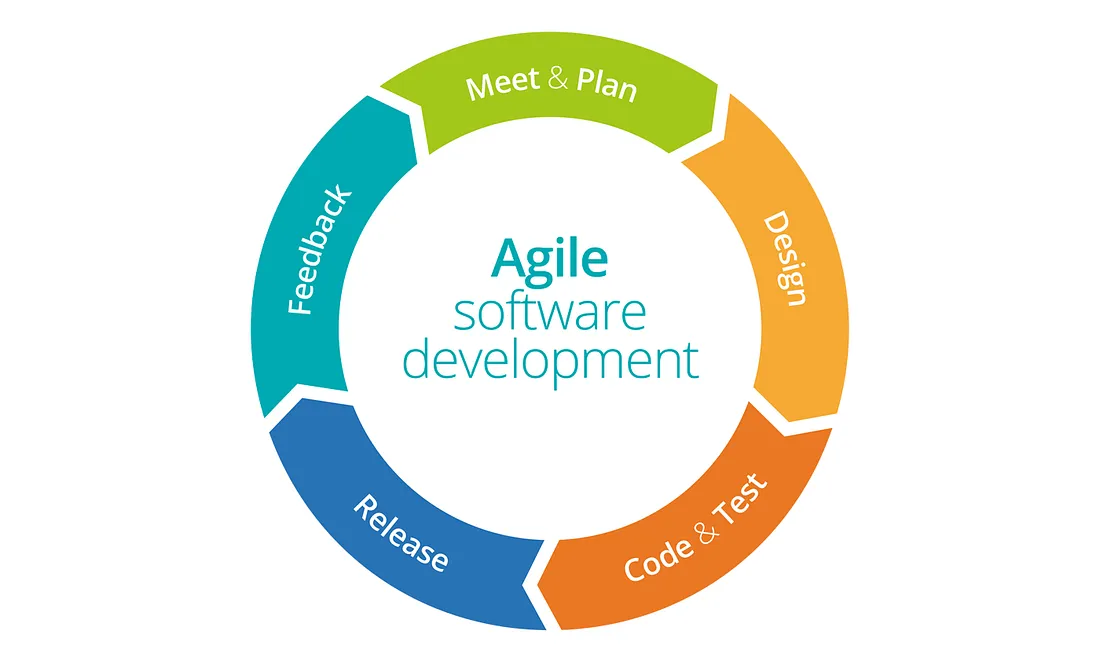
\includegraphics[width=0.7\linewidth]{assets/agile.png}}
    \caption{The Agile software development life cycle \cite{agile}}
\end{figure}

\Gls{agile} is an ideal approach for the \glsxtrshort{cuinspace} telemetry system because of the nature of development work
on an undergraduate design team. Members meet twice per week for 2 hours, where they complete as much development as
possible. Most members do not contribute outside of these meeting times (or do so infrequently) due to their course
load.

Additionally, prototypes must be available frequently throughout the year to test integration with other components in
development (such as the \glsxtrshort{srad} \glsxtrshortpl{pcb}). Frequent design iterations must also be available to
industry professionals, faculty and amateur rocketry competition organizers several times throughout the academic year
for their review. The limited timeline for deliverables and requirement for continuous delivery throughout the software
life cycle makes \gls{agile} an ideal choice.

Additionally, \gls{agile} includes instructions for how development should be carried out which integrates nicely with
the characteristics of a student design team. \Gls{agile} prescribes that a \gls{standup} lead each day of development,
which gives developers a chance to update others on their progress and address concerns. Members of the
\glsxtrshort{cuinspace} rocketry design team (especially those early in their undergraduate degree) become stuck on
development tasks because they lack the experience necessary to tackle problems on their own. The \gls{standup}
provides an opportunity for members to request help on tasks they are stuck on from other members or executives. Their
progress updates are also helpful for maintaining an up-to-date development timeline, which is critical due to the
short delivery times for software during the academic year.

\begin{figure}[H]
    \centerline{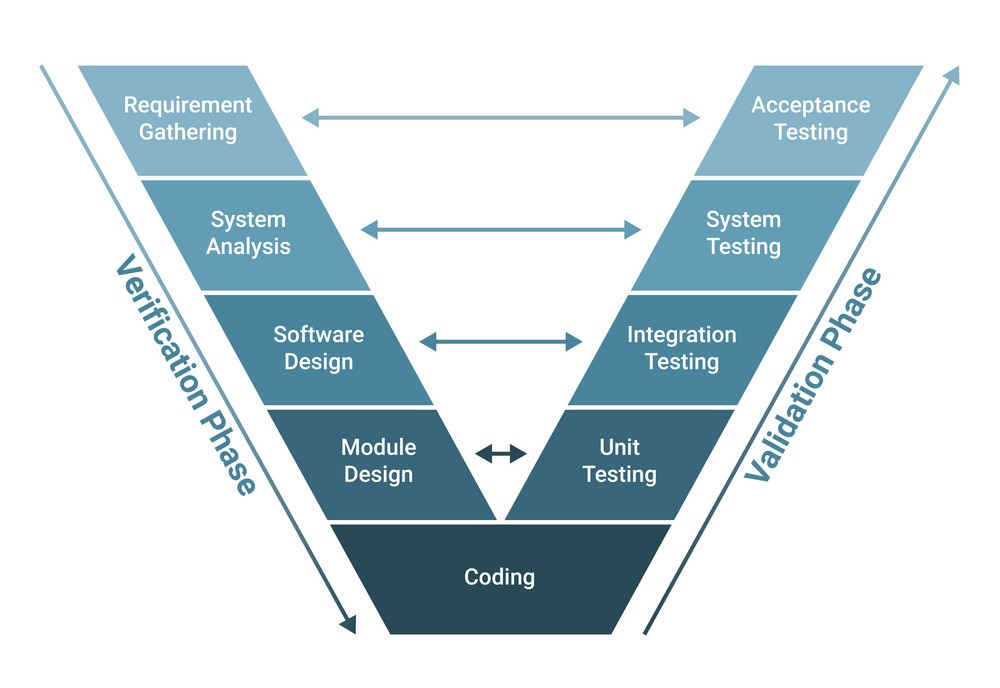
\includegraphics[width=0.7\linewidth]{assets/v-model.jpg}}
    \caption{The V-model software development life cycle \cite{vmodel}}
\end{figure}

The \gls{vmodel} also provides some inspiration for the development methodology of the telemetry system, as frequent
testing and prototyping is a hard requirement. The failure of \glsxtrshort{cuinspace}'s telemetry system in previous
years was due to a lack of continuous testing. This oversight led to a discovery of problems in range testing, which
was never solved and meant that no live telemetry data could be sent during flight. Utilizing the \gls{vmodel} will
require the telemetry system to have frequent prototypes used in testing, which will catch errors earlier in the
development cycle.

In addition to frequent testing, the \gls{vmodel} also prescribes requirements and architecture design to be completed
before implementation. Although this contradicts the \gls{agile} methodology and the nature of development on a student
design team, \glsxtrshort{cuinspace} plans to use this attribute of the \gls{vmodel} to encourage more detailed design
plans as early as possible in the year, before implementation is allowed to progress too far. Having a clearer plan
before the implementation phase begins gives members clearer direction with their tasks and reduces the probability of
having design incompatibilities after implementation is complete, requiring large, last-minute changes.

\subsection{Maintainability}

The \glsxtrshort{cuinspace} telemetry system software must be easily maintainable throughout high turnover of members
and an influx of interested members with limited software development knowledge. This is achieved with detailed
documentation, enforced software standards and division of responsibility between and within the software modules
discussed in \hyperref[s:modules]{section \ref{s:modules}}.

\subsubsection{Documentation}

In order to maintain and enforce detailed documentation of the telemetry system, auto-documentation generation using
Doxygen is enforced. See \hyperref[a:doxygen]{appendix \ref{a:doxygen}} for more information about Doxygen.

All of the software modules use a Doxygen configuration file which outputs warnings when code structures are left
undocumented (functions, C structs, enums, etc.). Doxygen documentation generation is automatically triggered when a
\glsxtrshort{pr} is merged into the module's respective codebase. This ensures that the documentation is always up to
date with the codebase.

In addition to automatic documentation generation on merges, GitHub repositories for the telemetry system modules are
set up to host the static \glsxtrshort{html} website created by Doxygen using \gls{githubpages}. This allows developers
to easily peruse existing documentation without requiring them to download it themselves or render the web-pages
locally.

Doxygen documentation is enforced using the \hyperref[a:javadoc]{JavaDoc style (more information in appendix
    \ref{a:javadoc})}. This style was selected because of its simple syntax, wide selection of information tags and because
it is taught in second year undergraduate engineering courses covering Java programming.

Documentation is required to be written wherever implementation occurs (C files for functions, header files for type
definitions, etc.). This avoids rebuilding all dependent source files when the documentation for a function prototype
is changed in a header file. \cite{doxygen-headers}

In addition to inline documentation for code, all modules mentioned in \hyperref[s:modules]{section \ref{s:modules}}
will come bundled with a help text document which can be invoked in the console with the \texttt{use} command. The help
document will include:

\begin{itemize}
    \setlength{\itemsep}{1pt}
    \setlength{\parskip}{0pt} \setlength{\parsep}{0pt}
    \item The module's version using \gls{semver} notation
    \item A description of the module's purpose
    \item Usage instructions for invocation
    \item A list of all command line options, positional arguments, their default values and the values they accept
    \item Example calls of the module
\end{itemize}

\subsubsection{Code Style}

All code is formatted according to a uniform \hyperref[a:clang-format]{clang-format (see appendix \ref{a:clang-format})
    for more information} configuration. This ensures that code formatting remains readable, and it also ensures that merge
conflicts due to developer formatting differences are avoided. Formatting is enforced via an automatic action on GitHub
which checks that the code adheres to the formatting guidelines before a \glsxtrshort{pr} can be merged.

A comprehensive set of compiler warnings is included in the build system for the telemetry software, which ensures that
common mistakes are caught at compile time (incorrect number of arguments to \texttt{printf}, unused declarations,
etc.). This ensures that code style is kept clean and free of bad practices. Warnings will be visible to developers
whenever they compile.

All code will be linted by GitHub actions using the \gls{qnx} compiler, \texttt{qcc}. This will ensure that compiler
warnings are detected before \glsxtrshort{pr}s are merged, giving developers the ability to fix their code before it
becomes part of the final product.

\subsection{Testing}

The development methodology chosen for the telemetry system places an emphasis on frequent prototyping. Testing is an
important part of the development methodology for validating prototypes continuously.

Developers will be responsible for writing unit tests for features that they implement. Unit tests will be executed
when \glsxtrshortpl{pr} are merged in order to verify that new changes do not break existing functionality. Tests that
are intentionally broken by new changes must come with a justification for the change and a rewrite/removal of the
affected tests.

Integration testing will be performed using shell scripts which can run on the Raspberry Pis. Using shell scripts
allows us to test our program in the real environment it will perform in, on actual hardware, including our
\glsxtrshort{srad} \glsxtrshortpl{pcb} which cannot be emulated in software without a considerable amount of effort.
Additionally, testing modules which are not hardware dependent is not possible automatically using GitHub's actions, as
the \gls{qnx} \glsxtrshort{rtos} kernel is fundamentally incompatible with Docker. \cite{docker-kernel-incompat}
